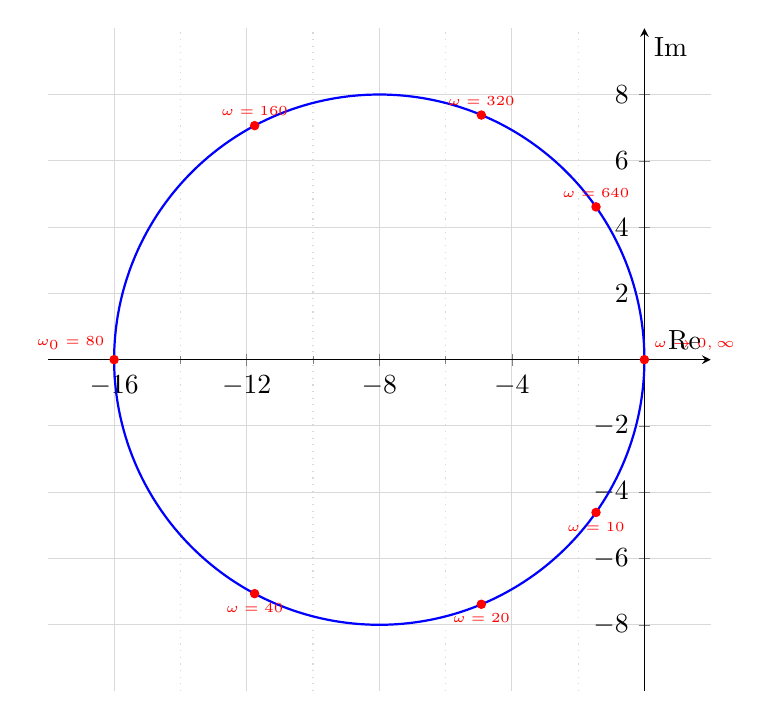
\begin{tikzpicture}
    \begin{axis}[
        xlabel={Re},
        ylabel={Im},
        grid=both,
        width=10cm,
        height=10cm,
        xmin=-18.0, xmax=2.0,
        ymin=-10.0, ymax=10.0,
        axis lines=middle,
        minor tick num=1,
        major grid style={solid, gray!30},
        minor grid style={dotted, gray!30},
        clip=false,
        xtick={-16, -12, -8, -4, 0},
        ytick={-8, -6, -4, -2, 2, 4, 6, 8},
    ]
        % Curva polar paramétrica usando parametrización geométrica (circulo perfecto)
        \addplot[blue, thick, smooth, domain=0:360, samples=180] ({
            -8 + 8 * cos(x)
        }, {
            8 * sin(x)
        });
        
        % Puntos notables
        \addplot[only marks, red, mark=*, mark size=1.5pt] coordinates {
            (0,0)
            (-1.46,-4.61)
            (-4.92,-7.38)
            (-11.76,-7.06)
            (-16,0)
            (-11.76,7.06)
            (-4.92,7.38)
            (-1.46,4.61)
        };
        
        \node[above right, font=\tiny, text=red] at (axis cs:0,0) {$\omega \to 0, \infty$};
        \node[below, font=\tiny, text=red] at (axis cs:-1.46,-4.61) {$\omega=10$};
        \node[below, font=\tiny, text=red] at (axis cs:-4.92,-7.38) {$\omega=20$};
        \node[below, font=\tiny, text=red] at (axis cs:-11.76,-7.06) {$\omega=40$};
        \node[above left, font=\tiny, text=red] at (axis cs:-16,0) {$\omega_0=80$};
        \node[above, font=\tiny, text=red] at (axis cs:-11.76,7.06) {$\omega=160$};
        \node[above, font=\tiny, text=red] at (axis cs:-4.92,7.38) {$\omega=320$};
        \node[above, font=\tiny, text=red] at (axis cs:-1.46,4.61) {$\omega=640$};
    \end{axis}
\end{tikzpicture}
